\chapter{Gestión del proyecto}\label{chap:project_management}

A lo largo del proyecto se establecieron procesos y herramientas que permiten el desarrollo del mismo con efectividad. Desde la gestión y planificación de tareas hasta herramientas de desarrollo, versionado de código, gestión de la documentación, almacenamiento de archivos compartidos, diagramas, etc. En este capítulo se detallan todas las herramientas y procesos de trabajo utilizados; las actividades del proyecto organizadas en sus distintas etapas; y por último, un reporte de los costos que implicó el desarrollo del proyecto. 

\section{Actividades y cronología}\label{section:project-activites}

Durante el transcurso del proyecto, se realizaron diversas actividades para alcanzar los resultados obtenidos. Estas actividades se organizaron en etapas, las cuales se llevaron adelante con un orden específico planificado con anterioridad. En esta sección se detallan estas actividades, la duración de las mismas y cómo fueron organizadas. 

Las actividades principales llevadas a cabo durante el proyecto fueron: 

\begin{itemize}
    \item Relevamiento inicial: Comprender la problemática, conocer el equipo de trabajo, definir el objetivo del proyecto y el alcance a grandes rasgos.
    \item Estado del arte: Investigación sobre los avances en el área de \gls{gait_analysis}. Revisión sistemática de la literatura (SLR).
    \item Compra de dispositivos IMU y coordinación de envío desde E.E.U.U.
    \item Estudio de tecnología Android.
    \item PoC: Prueba de conceptos para mitigación de riesgos técnicos. 
    \item Desarrollo de la aplicación:
    \begin{itemize}
        \item Análisis: Alcance, especificación detallada y casos de uso
        \item Diseño: Diagrama de clases. Interfaz y experiencia de usuario. 
        \item Implementación de la aplicación Android.
        \item Revisión de código entre pares.
        \item Pruebas del sistema: exploratorias, funcionales y no funcionales. 
    \end{itemize}
    \item SABI 2020: Congreso de bioingeniería. Marzo 2020, Piriápolis.
        \begin{itemize}
            \item Desarrollo de un artículo científico para REVISTA ARGENTINA DE BIOINGENIERÍA. 
            \item Presentación y exposición de PARKIBIP en congreso (Fig. \ref{fig:sabi2020})
        \end{itemize}
    \item Análisis de resultados 
    \item Gestión del proyecto
        \begin{itemize}
            \item Planificación
            \item Gestión de tareas
            \item Reuniones con tutores
	        \item Reuniones con fisioterapeutas
	        \item Coordinación para visita a sesiones de fisioterapia
	        \item Gestión con Asociación Uruguaya de Parkinson para pruebas con integrantes voluntarios 
        \end{itemize} 
    \item Documentación del proyecto
\end{itemize}

\newpage

\begin{figure}[H]

\includegraphics[width=\textwidth]{TESIS/imagenes/chap07/SABI-2020.jpeg}
\caption{ Exposición de PARKIBIP en Congreso de Bioingeniería y Jornadas de Ingeniería Clínica SABI 2020. De izquierda a derecha: Carlos Huerta y Samuel Sainz. Marzo 2020. Argentino Hotel, Piriápolis, Uruguay. }
\label{fig:sabi2020}
\end{figure}

El proyecto comenzó en Setiembre de 2018 y se finalizó en Diciembre de 2020. En el diagrama de Gantt de la figura Fig. \ref{fig:gantt-parkibip} se muestra el orden cronológico en el que se realizaron las actividades. Este diagrama resulta útil para entender la duración de las tareas en comparación con la duración del proyecto final; así como para poder comparar la duración de una tarea con respecto a la otra. Además, permite ver visualmente como se organizaron las actividades del proyecto de principio a fin. 

\newpage

\begin{figure}[H]
\hspace{-3.0cm}
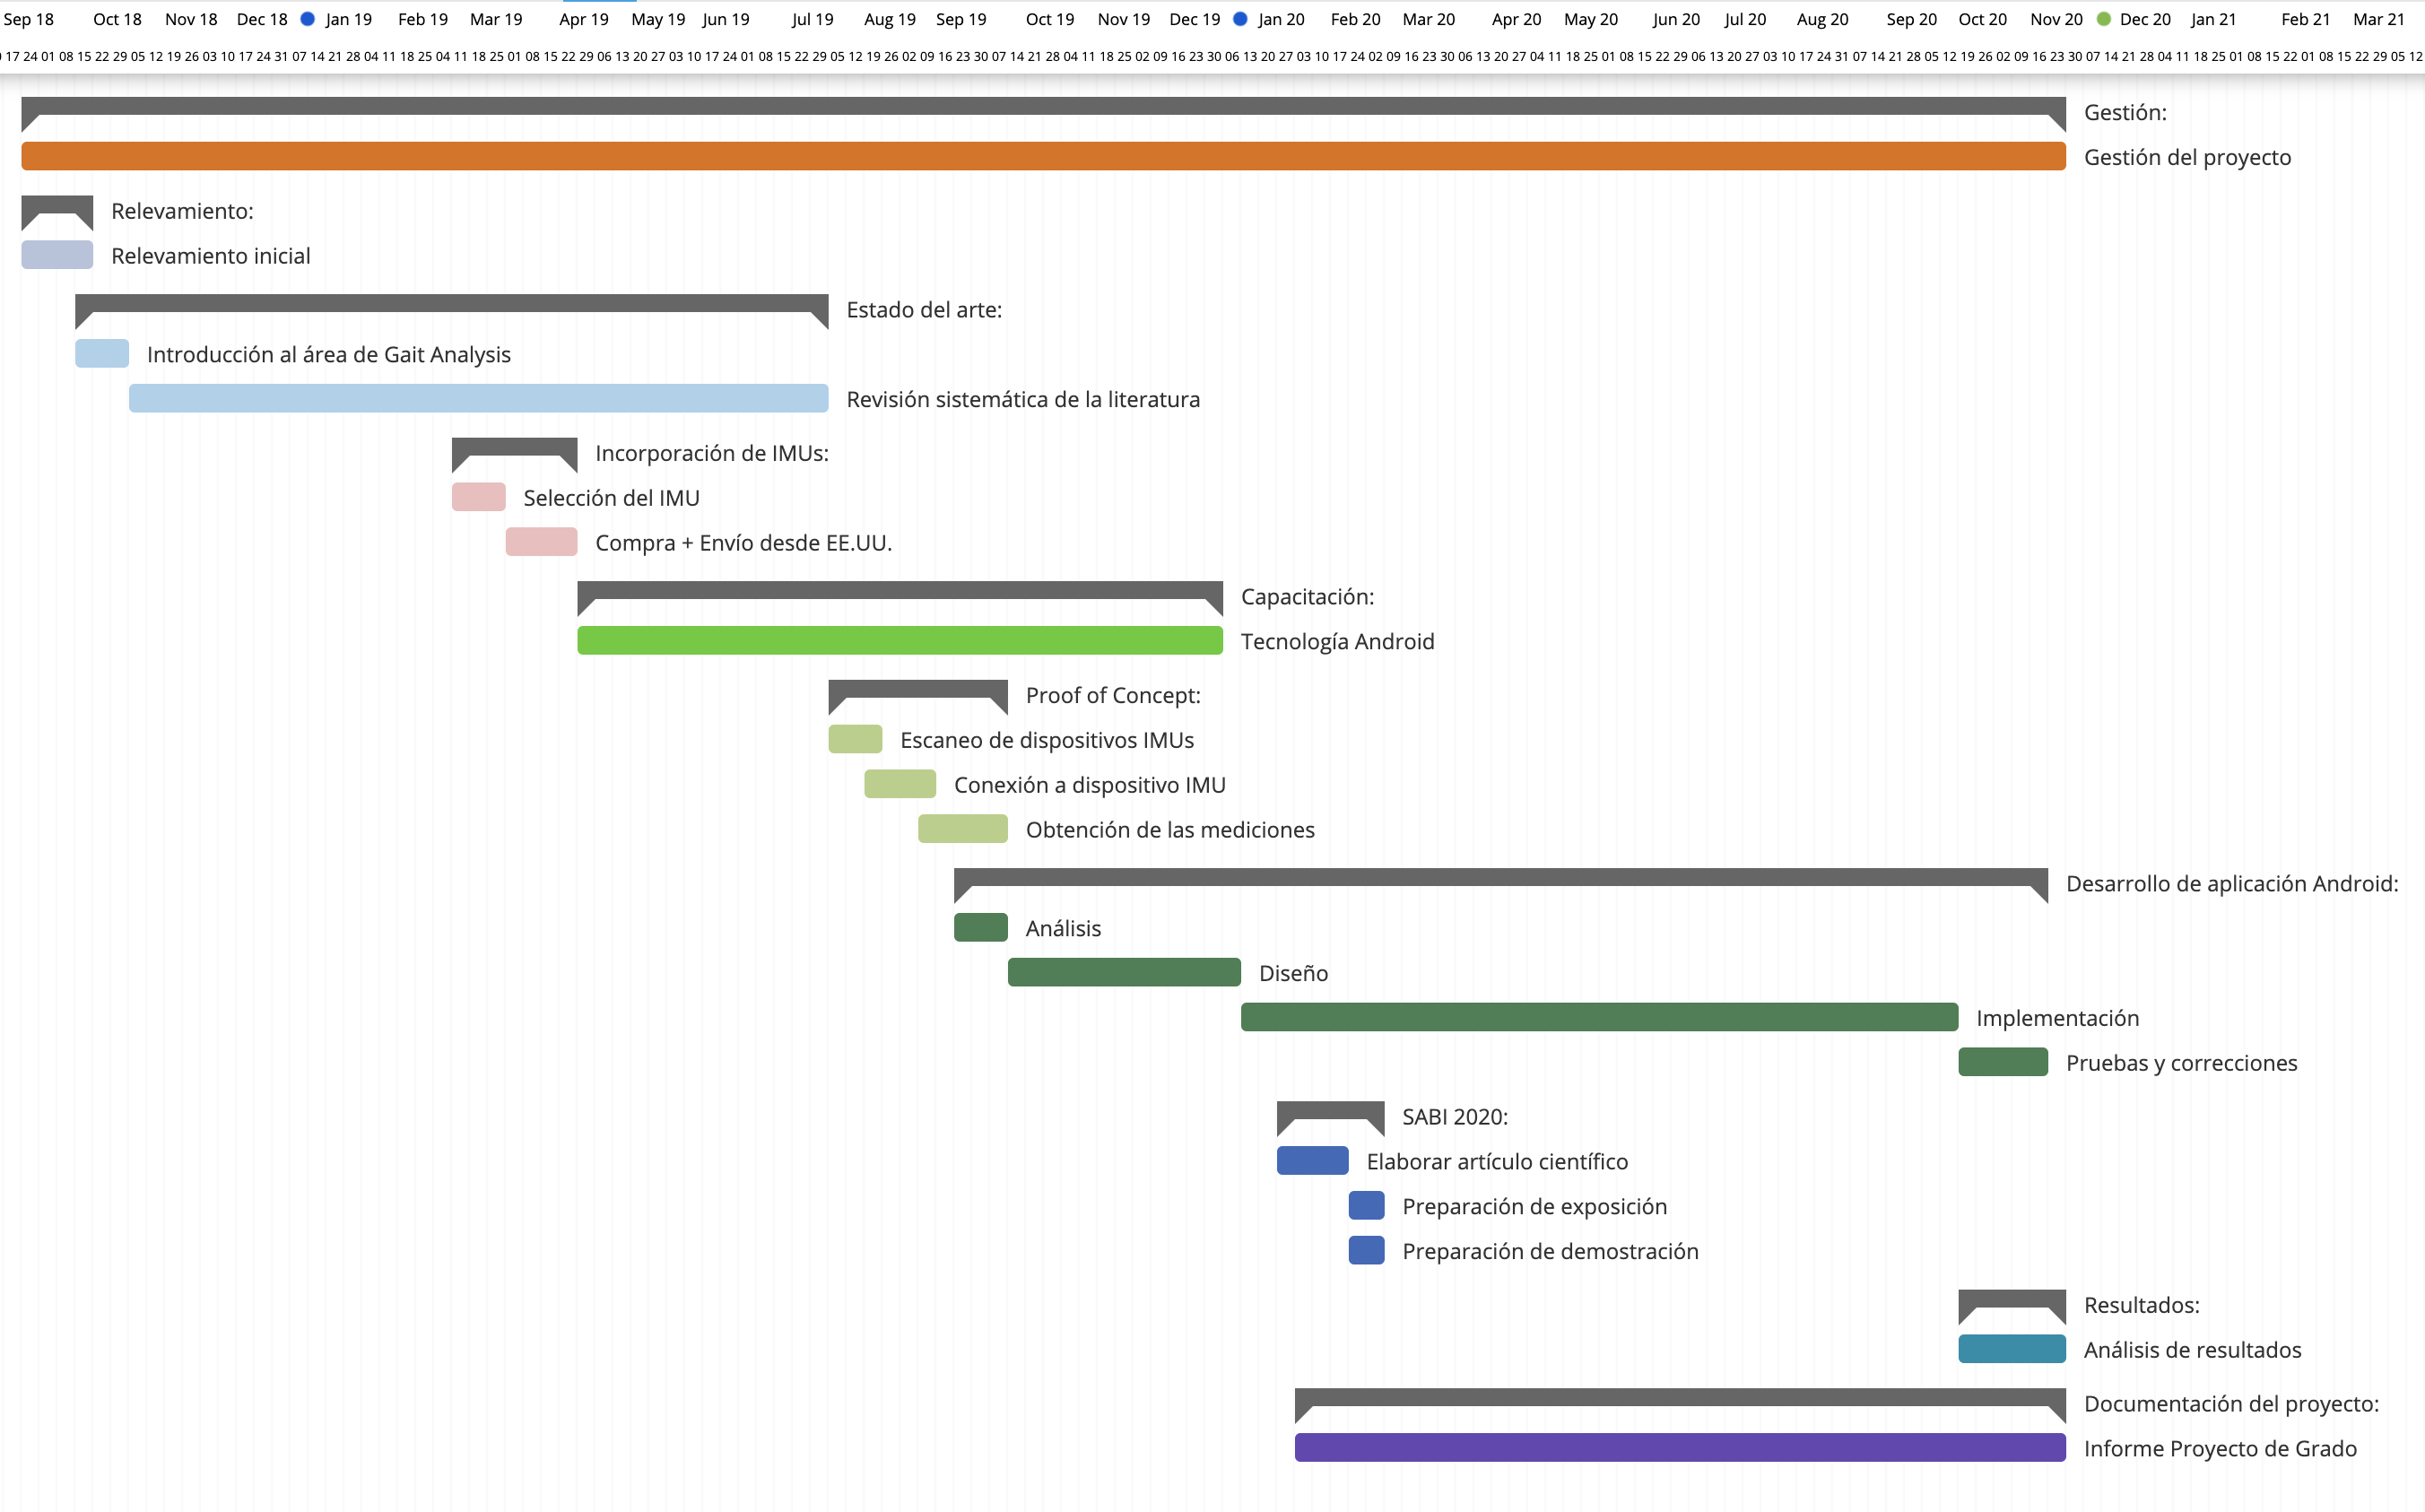
\includegraphics[clip,width=1.32 \columnwidth]{TESIS/imagenes/chap07/gantt-parkibip.png}
\caption{Diagrama de Gantt. Expone las actividades realizadas durante el proyecto PARKIBIP desde el inicio del proyecto en Setiembre de 2018 hasta el final del proyecto en Noviembre de 2020. }
\label{fig:gantt-parkibip}
\end{figure}

\section{Reporte de costos}

Con el objetivo de determinar los costos del proyecto, en una primera instancia se deben evaluar las inversiones de horas-persona. Las horas-personas son la unidad de medida que se emplea en gestión de proyectos para medir los esfuerzos necesarios para completar una tarea. Una hora-hombre equivale al trabajo completado en una hora de esfuerzo ininterrumpido por un trabajador. 

La tabla Tab. \ref{TAB:expenses} resume la inversión de horas en el proyecto PARKIBIP mediante los campos: (i) costo hora-persona de cada uno de los integrantes -usando la media de la industria-, (ii) el total de horas invertidas en el proyecto y (iii) el costo total para cada persona del equipo. Considerando todos los elementos, en total se invirtieron 2.334 horas calificadas del equipo multidisciplinario, con un costo total que asciende a los USD 111.195.

\begin{table}[H]
\caption{Resumen de horas dedicadas por participante del proyecto con su respectivo costo, teniendo en cuenta el rol de la persona.}
\centering
\hspace*{-2.5cm}%
\begin{tabular}{|c|c|p{2.0cm}|p{2.7cm}|p{2.5cm}|}
\hline
\textbf{Persona} & \textbf{Rol} & \textbf{Horas dedicadas} & \textbf{Costo hora-persona (USD)} & \textbf{Costo total (USD)}  \\ \hline
Est. Ing. en Computación 1 & Ingeniero & 1.084 & 45 & 48.780 \\ \hline
Est. Ing. en Computación 2 & Ingeniero & 1.063 & 45 & 47.835 \\ \hline
Est. de Fisioterapia & Fisioterapeuta & 50 & 45 & 2.250 \\ \hline
Tutor de Proyecto de Grado & \gls{product_owner} & 137 & 90 & 12.330 \\ \hline
\end{tabular}
\hspace*{-1cm}
\label{TAB:expenses}
\end{table}

Se analizó, además, la evolución de la dedicación horaria a lo largo del proyecto a partir de las actividades detalladas en la sección \nameref{section:project-activites}. La figura Fig. \ref{fig:dedication} expone una serie temporal en meses con dicha evolución en horas-persona. Estudiando el gráfico, se puede apreciar: (i) una línea de tendencia ascendente desde el inicio del proyecto hacia su finalización, (ii) momentos de bajo rendimiento, en general, para los meses enero e inicio de febrero (e.g. debido a ocio, parciales o exámenes), (iii) picos máximos en los meses de marzo y noviembre de 2020 -correspondiente a SABI 2020 y a la finalización del proyecto-.

\begin{figure}[h!]
\hspace*{-2.9cm}%
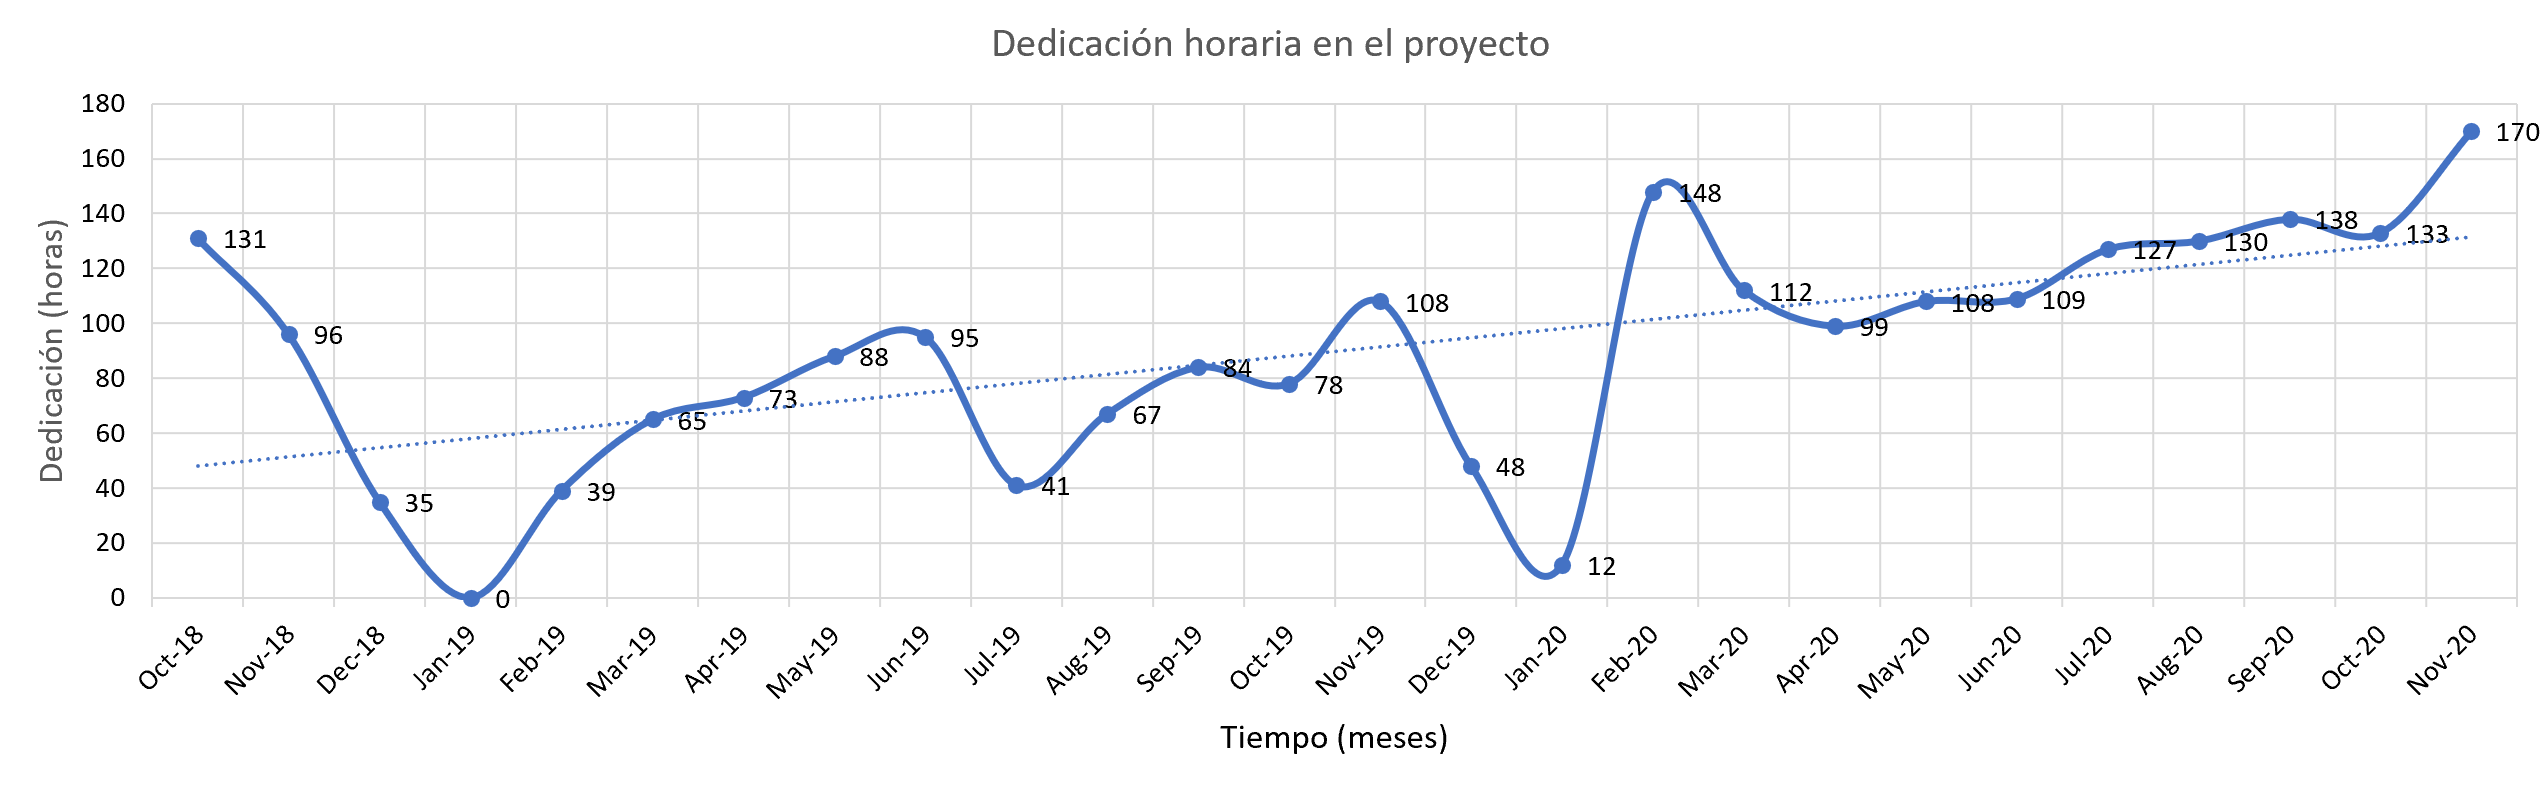
\includegraphics[clip,width=1.4 \columnwidth]{TESIS/imagenes/chap07/dedication-parkibip.PNG}
\caption{Evolución en meses de la dedicación horaria en el proyecto.}
\label{fig:dedication}
\end{figure}

Por otro lado, para determinar de qué forma se invirtió el esfuerzo en las distintas actividades del proyecto, fueron establecidos seis centros de costo correspondientes a las principales actividades. Así, con el propósito de facilitar la comprensión de los diferentes gastos requeridos por PARKIBIP, se propone la figura Fig. \ref{fig:dedication-costs}, la cual presenta una serie temporal en meses con la distribución horaria por centro de costo. 

\begin{figure}[h!]
\hspace*{-2.9cm}%
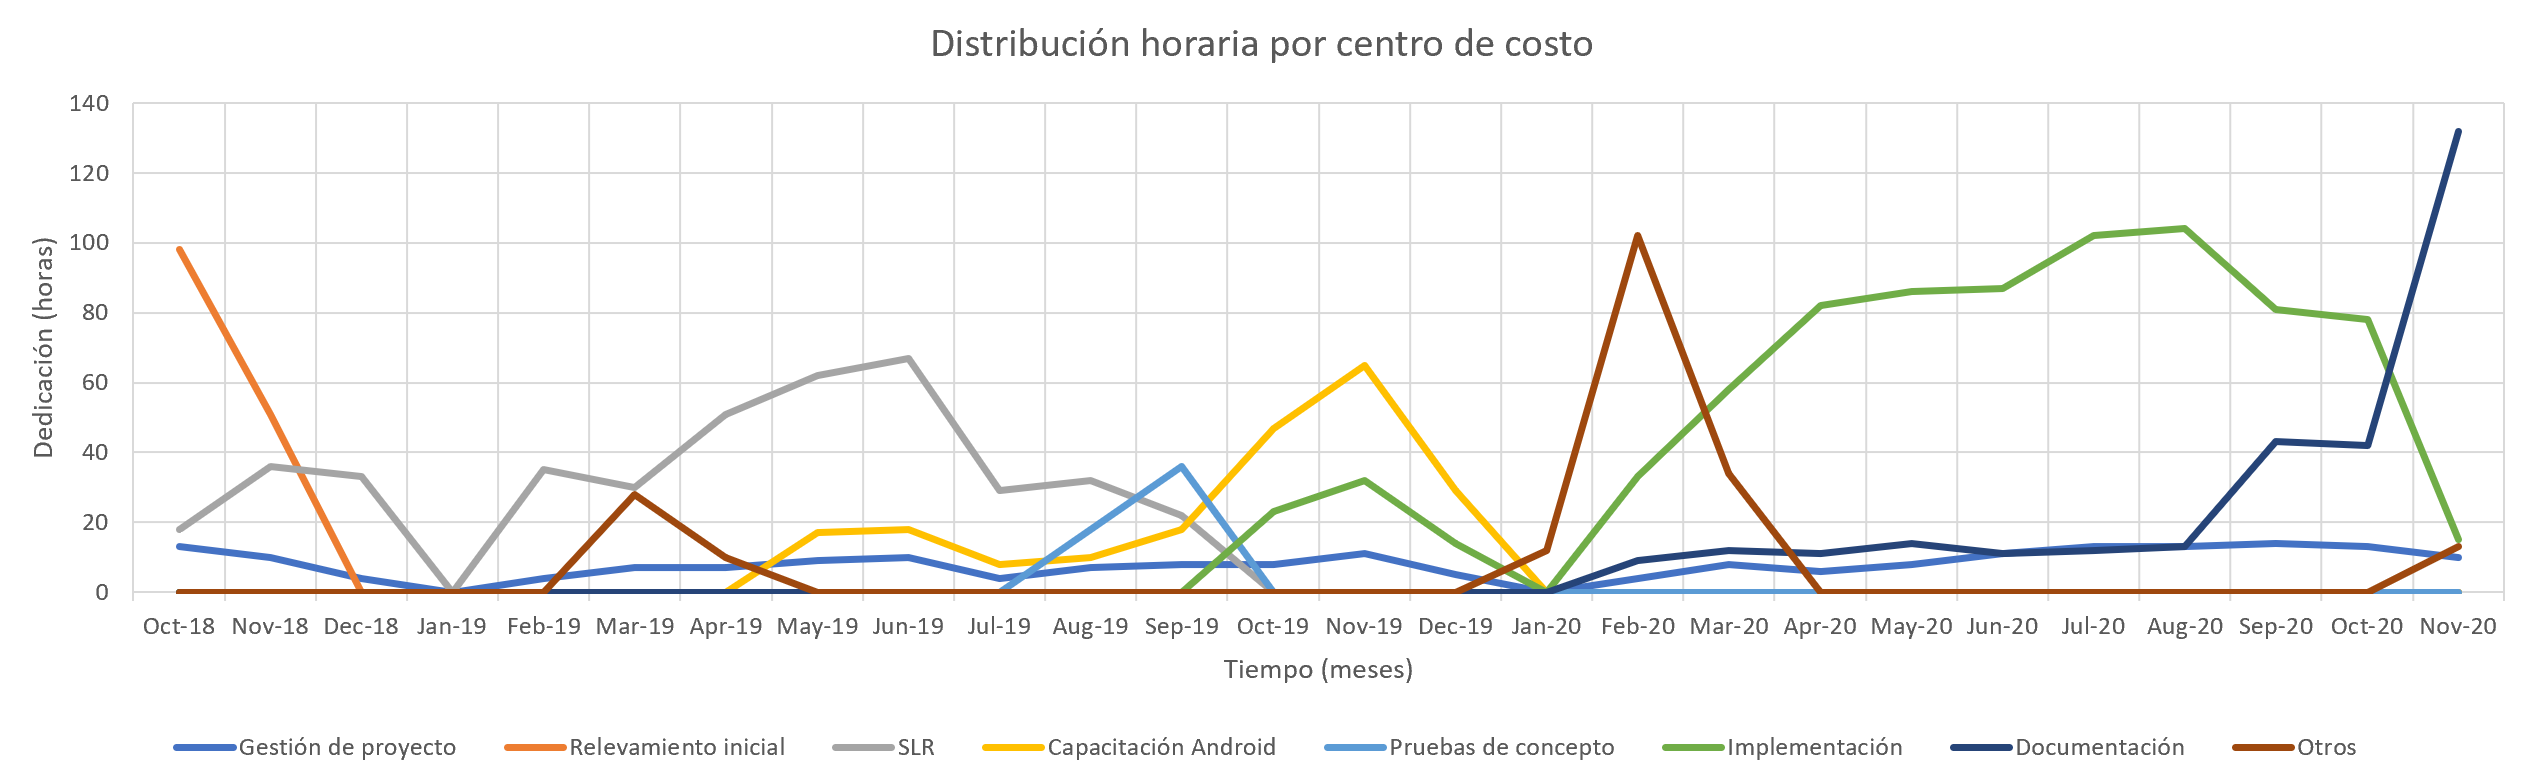
\includegraphics[clip,width=1.4 \columnwidth]{TESIS/imagenes/chap07/dedication-costs.PNG}
\caption{Serie temporal en meses con la distribución horaria por centro de costo.}
\label{fig:dedication-costs}
\end{figure}

La tabla Tab. \ref{TAB:dedication-per-center} resume la información de la dedicación horaria por centro de costo, mostrando: (i) la cantidad de horas para cada centro de costos, (ii) el porcentaje del total de horas que fue dedicado a cada actividad.

\begin{table}[H]
\caption{Resumen de horas dedicadas por actividad del proyecto, correspondientes a los distintos centros de costo.}
\centering
\hspace*{-2.5cm}%
\begin{tabular}{|c|c|c|}
\hline
\textbf{Centro de costo} & \textbf{Horas dedicadas} & \textbf{Porcentaje sobre total de horas} \\ \hline
Gestión de proyecto & 207 & 8.88\% \\ \hline
Relevamiento inicial & 149 & 6.39\% \\ \hline
Revisión Sistemática (SLR) & 415 & 17.81\% \\ \hline
Capacitación Android & 212 & 9.10\% \\ \hline
Pruebas de concepto	& 54 & 2.32\% \\ \hline
Implementación & 795 & 34.12\% \\ \hline
Documentación & 299 & 12.83\% \\ \hline
Otros\footnotemark & 199 & 8.54\% \\ \hline
\end{tabular}
\hspace*{-1cm}
\label{TAB:dedication-per-center}
\end{table}

\footnotetext{Dentro del centro de costos \textit{Otros}, se incluyen actividades con una inversión horaria menor, como lo son: Selección y compra de IMUs, Preparación y participación en SABI 2020, entre otras.}

Por otra parte, en adición al costo calculado según la dedicación del equipo, se deben contemplar también otras expensas como: 

\begin{itemize}
    \item Inscripción a congreso SABI 2020: 90 USD (45 USD por cada estudiante)
    \item Viáticos de viaje a congreso: 360 USD (180 USD por estudiante)
    \item Dispositivos IMU: 190 USD (95 USD cada uno) 
    \item Bandas para fijación de IMU: 10 USD
    \item Envío de los IMU desde EE.UU: 35 USD
\end{itemize}

Estos gastos adicionales suman un monto de USD 685. Por lo tanto, en base a la estimación de horas y costos realizadas, \textbf{el proyecto presenta un costo total aproximado de USD 111.880}.

\section{Gestión de tareas}
% Trello 
La organización del \gls{backlog} de tareas es importante para la gestión del proyecto. Trello (© 2020 Trello, Help Scout) es una herramienta simple y gratuita para administrar las actividades de un proyecto. Se basa principalmente en un tablero de tarjetas, en el que cada tarjeta representa una tarea a ser realizada en el proyecto. La herramienta permite crear listas -en forma de columnas-, en donde las tarjetas pueden ser agregadas, y así organizar el trabajo según cualidades definidas por los administradores del proyecto. Trello, tiene como principal ventaja la capacidad de brindar fácilmente una visión sobre el estado del proyecto: el trabajo que fue realizado, el que está en curso y el que se encuentra pendiente; así como las personas involucradas en el desarrollo de cada tarea, entre otras propiedades. 

Conforme a lo mencionado, el tablero de PARKIBIP fue dividido en 7 listas ordenadas de tareas:

\begin{itemize}
    \item Tareas relacionadas a la gestión del proyecto
    \item Tareas referidas al desarrollo del informe
    \item Tareas de implementación del sistema de software 
    \item Tareas en curso 
    \item Pendientes de evaluación de calidad
    \item Tareas finalizadas
\end{itemize}

Asimismo, Trello permite agregar etiquetas a las tarjetas -de diversos colores-, así distinguirlas fácilmente dentro del tablero. En PARKIBIP, las etiquetas se emplearon para diferenciar el tipo de tarea: planificación, análisis, diseño, implementación, testing o error de sistema (bug). 

Con el fin de estandarizar la gestión del proyecto, se estableció la información que debe ser agregada en la creación de cada tarjeta o actividad:

\begin{itemize}
    \item Nombre y descripción de la tarea 
    \item Persona asignada a la tarea -condición obligatoria para la ejecución de actividad-
    \item Etiquetas que establezcan el tipo de tarea 
    \item Utilizar la funcionalidad de ``checklist'' si la tarea lo amerita 
    \item En caso que corresponda agregar información extra sobre el resultado, emplear comentarios
\end{itemize}

La figura Fig. \ref{fig:admin_project} resume la metodología empleada para la gestión del trabajo. 

\begin{figure}[H]
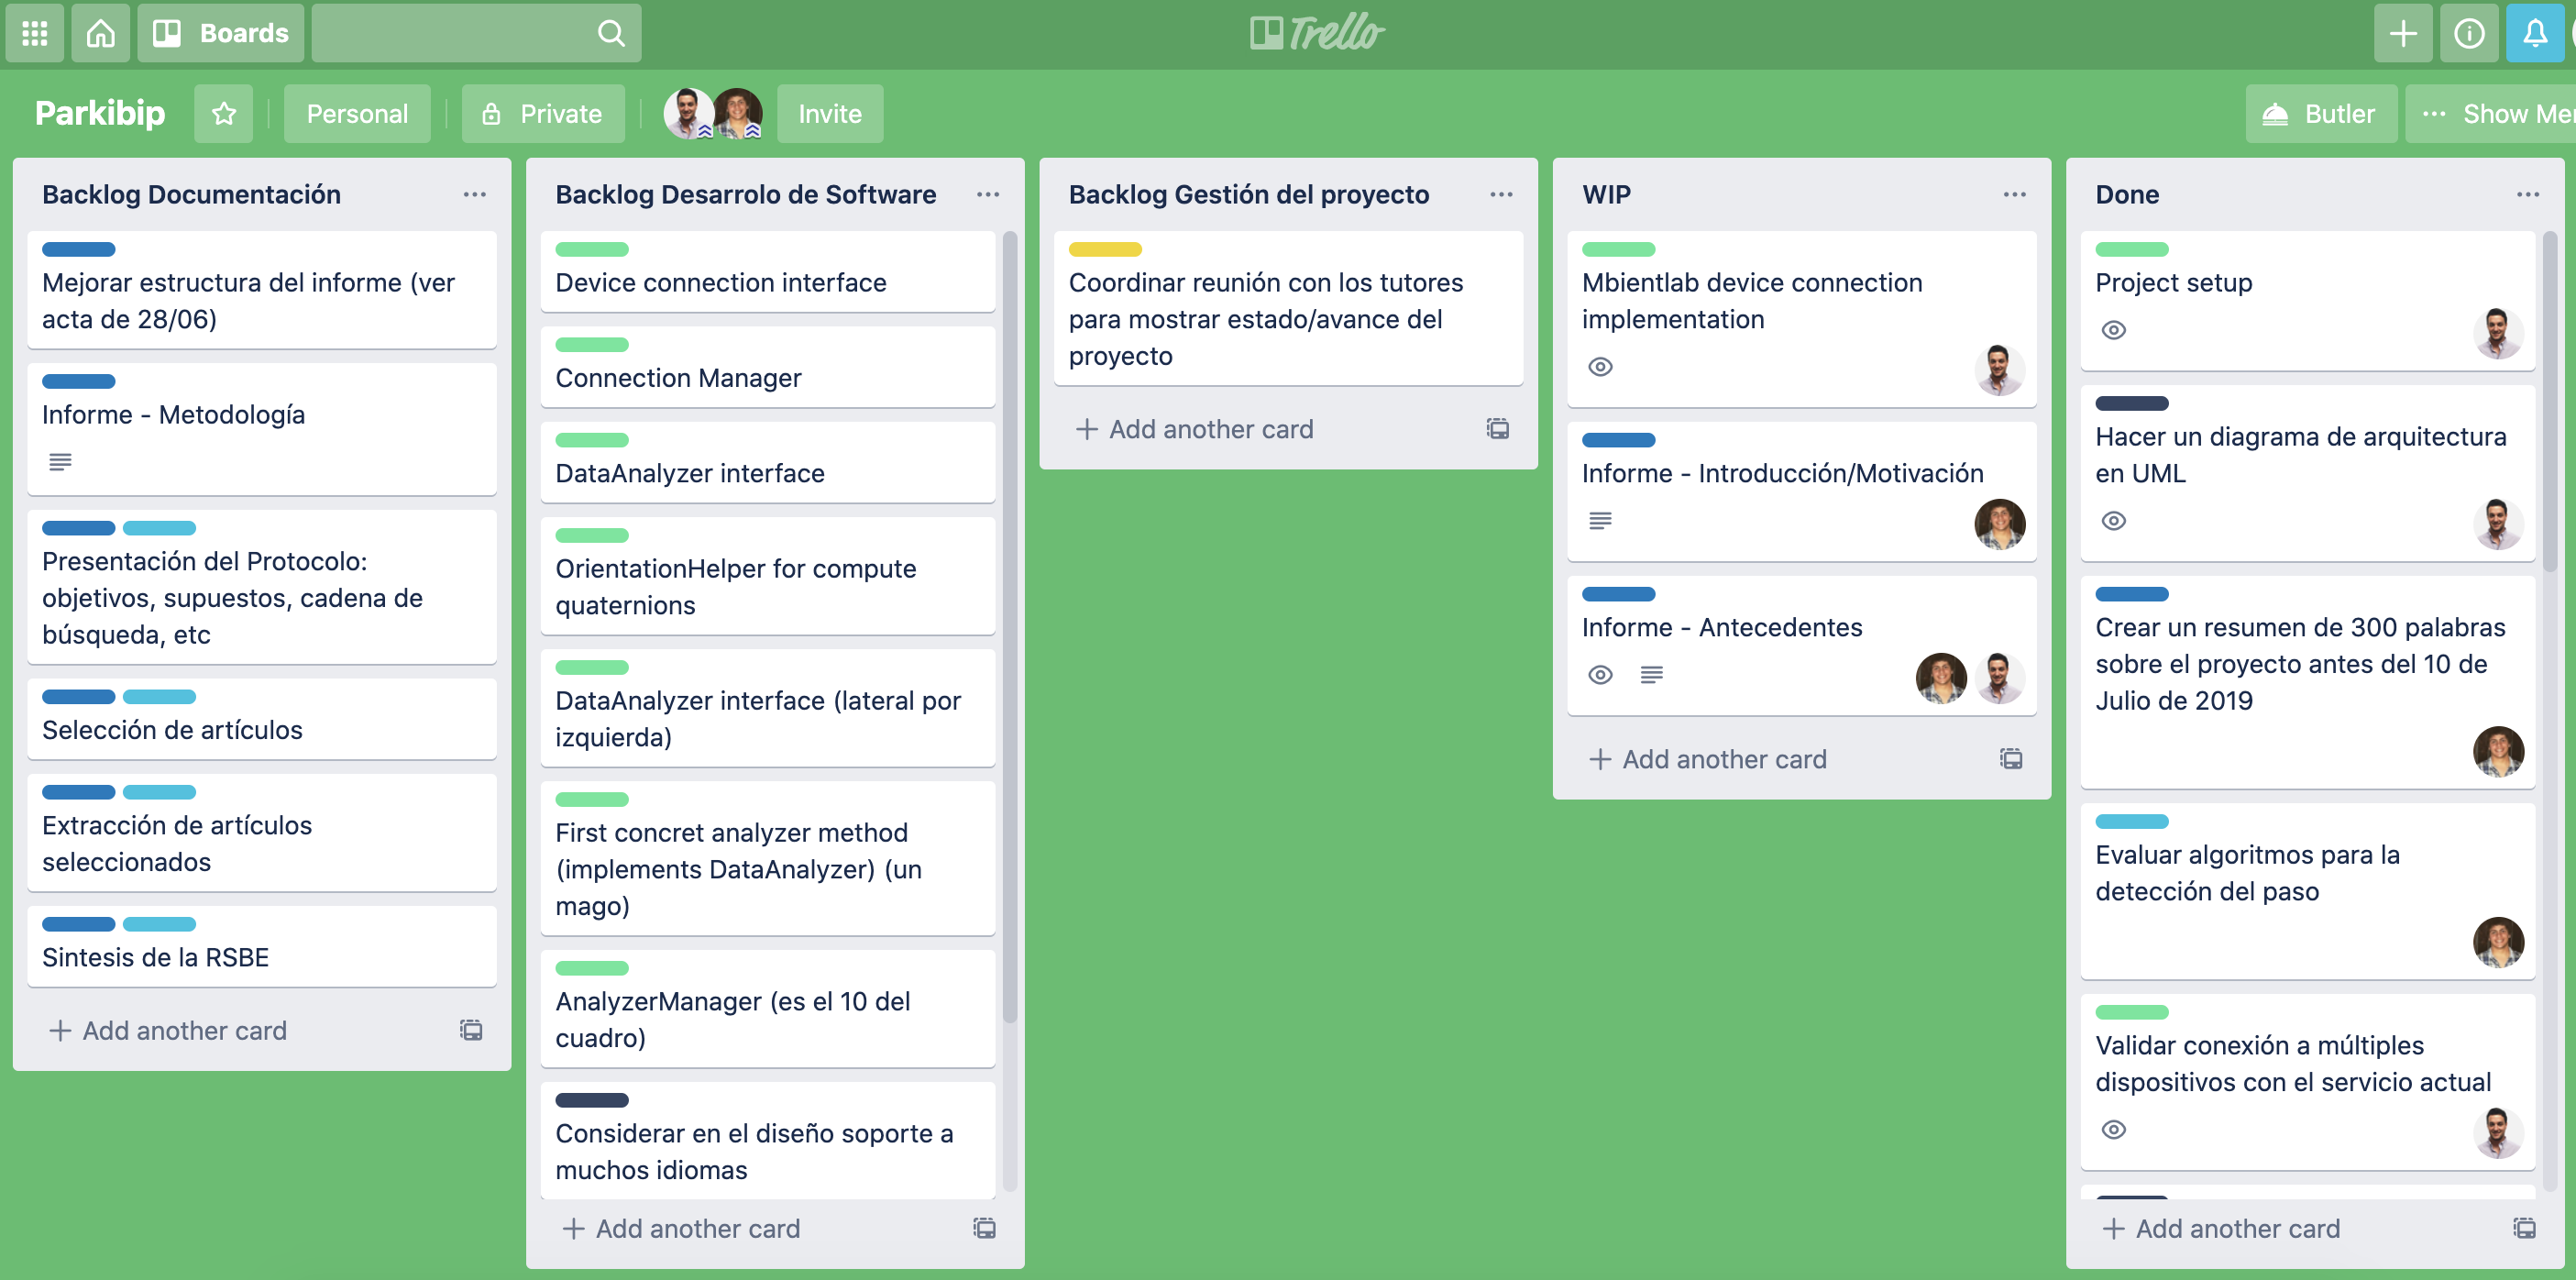
\includegraphics[width=\textwidth]{TESIS/imagenes/chap04/trello.png}
\caption{ Herramienta de gestión de proyecto. }
\label{fig:admin_project}
\end{figure}

% Google Drive & Sheets 

\section{Administración bibliográfica}

Resulta fundamental para analizar la literatura recopilada en el área de estudio y para desarrollar el estado del arte del proyecto, emplear una herramienta que brinde facilidades para la administración de las referencias bibliográficas. El gestor clásico Mendeley (© 2009-2013 Mendeley Ltd., Elsevier), fue la herramienta elegida por el equipo de trabajo para dicho fin. Toda la bibliografía seleccionada como relevante se agregó a la plataforma en un proyecto compartido por los investigadores. 
En una SLR, un gestor bibliográfico es de gran utilidad para administrar el inmenso volumen de estudios científicos. Así, la herramienta Mendeley fue ampliamente utilizada en las etapas de selección y extracción de artículos de la SLR. A continuación, se destacan las principales funcionalidades de la herramienta utilizadas en el proyecto: 

\begin{itemize}
    \item Creación de un proyecto compartido para el almacenamiento de los artículos en la nube
    \item Centralizar la evidencia recopilada para una mejor trazabilidad y organización
    \item Extensión del explorador de internet para la importación de artículos al proyecto
    \item Generación de citas de los artículos en formato ``bibtex'' utilizado en este documento 
    \item Subrayar, efectuar notas y comentarios con el fin de destacar sentencias dentro del artículo -visibles para el resto de los integrantes del proyecto- 
\end{itemize}

La ilustración Fig. \ref{fig:admin_references} permite visualizar la herramienta aplicada a el proyecto PARKIBIP, su organización configurable (i.e. datos básicos: autores, titulo, año de publicación, fuente) y algunas funcionalidades. Se administraron y analizaron aproximadamente 60 estudios en la librería -no se contabilizan los artículos indagados en otra herramienta-.

\begin{figure}[H]
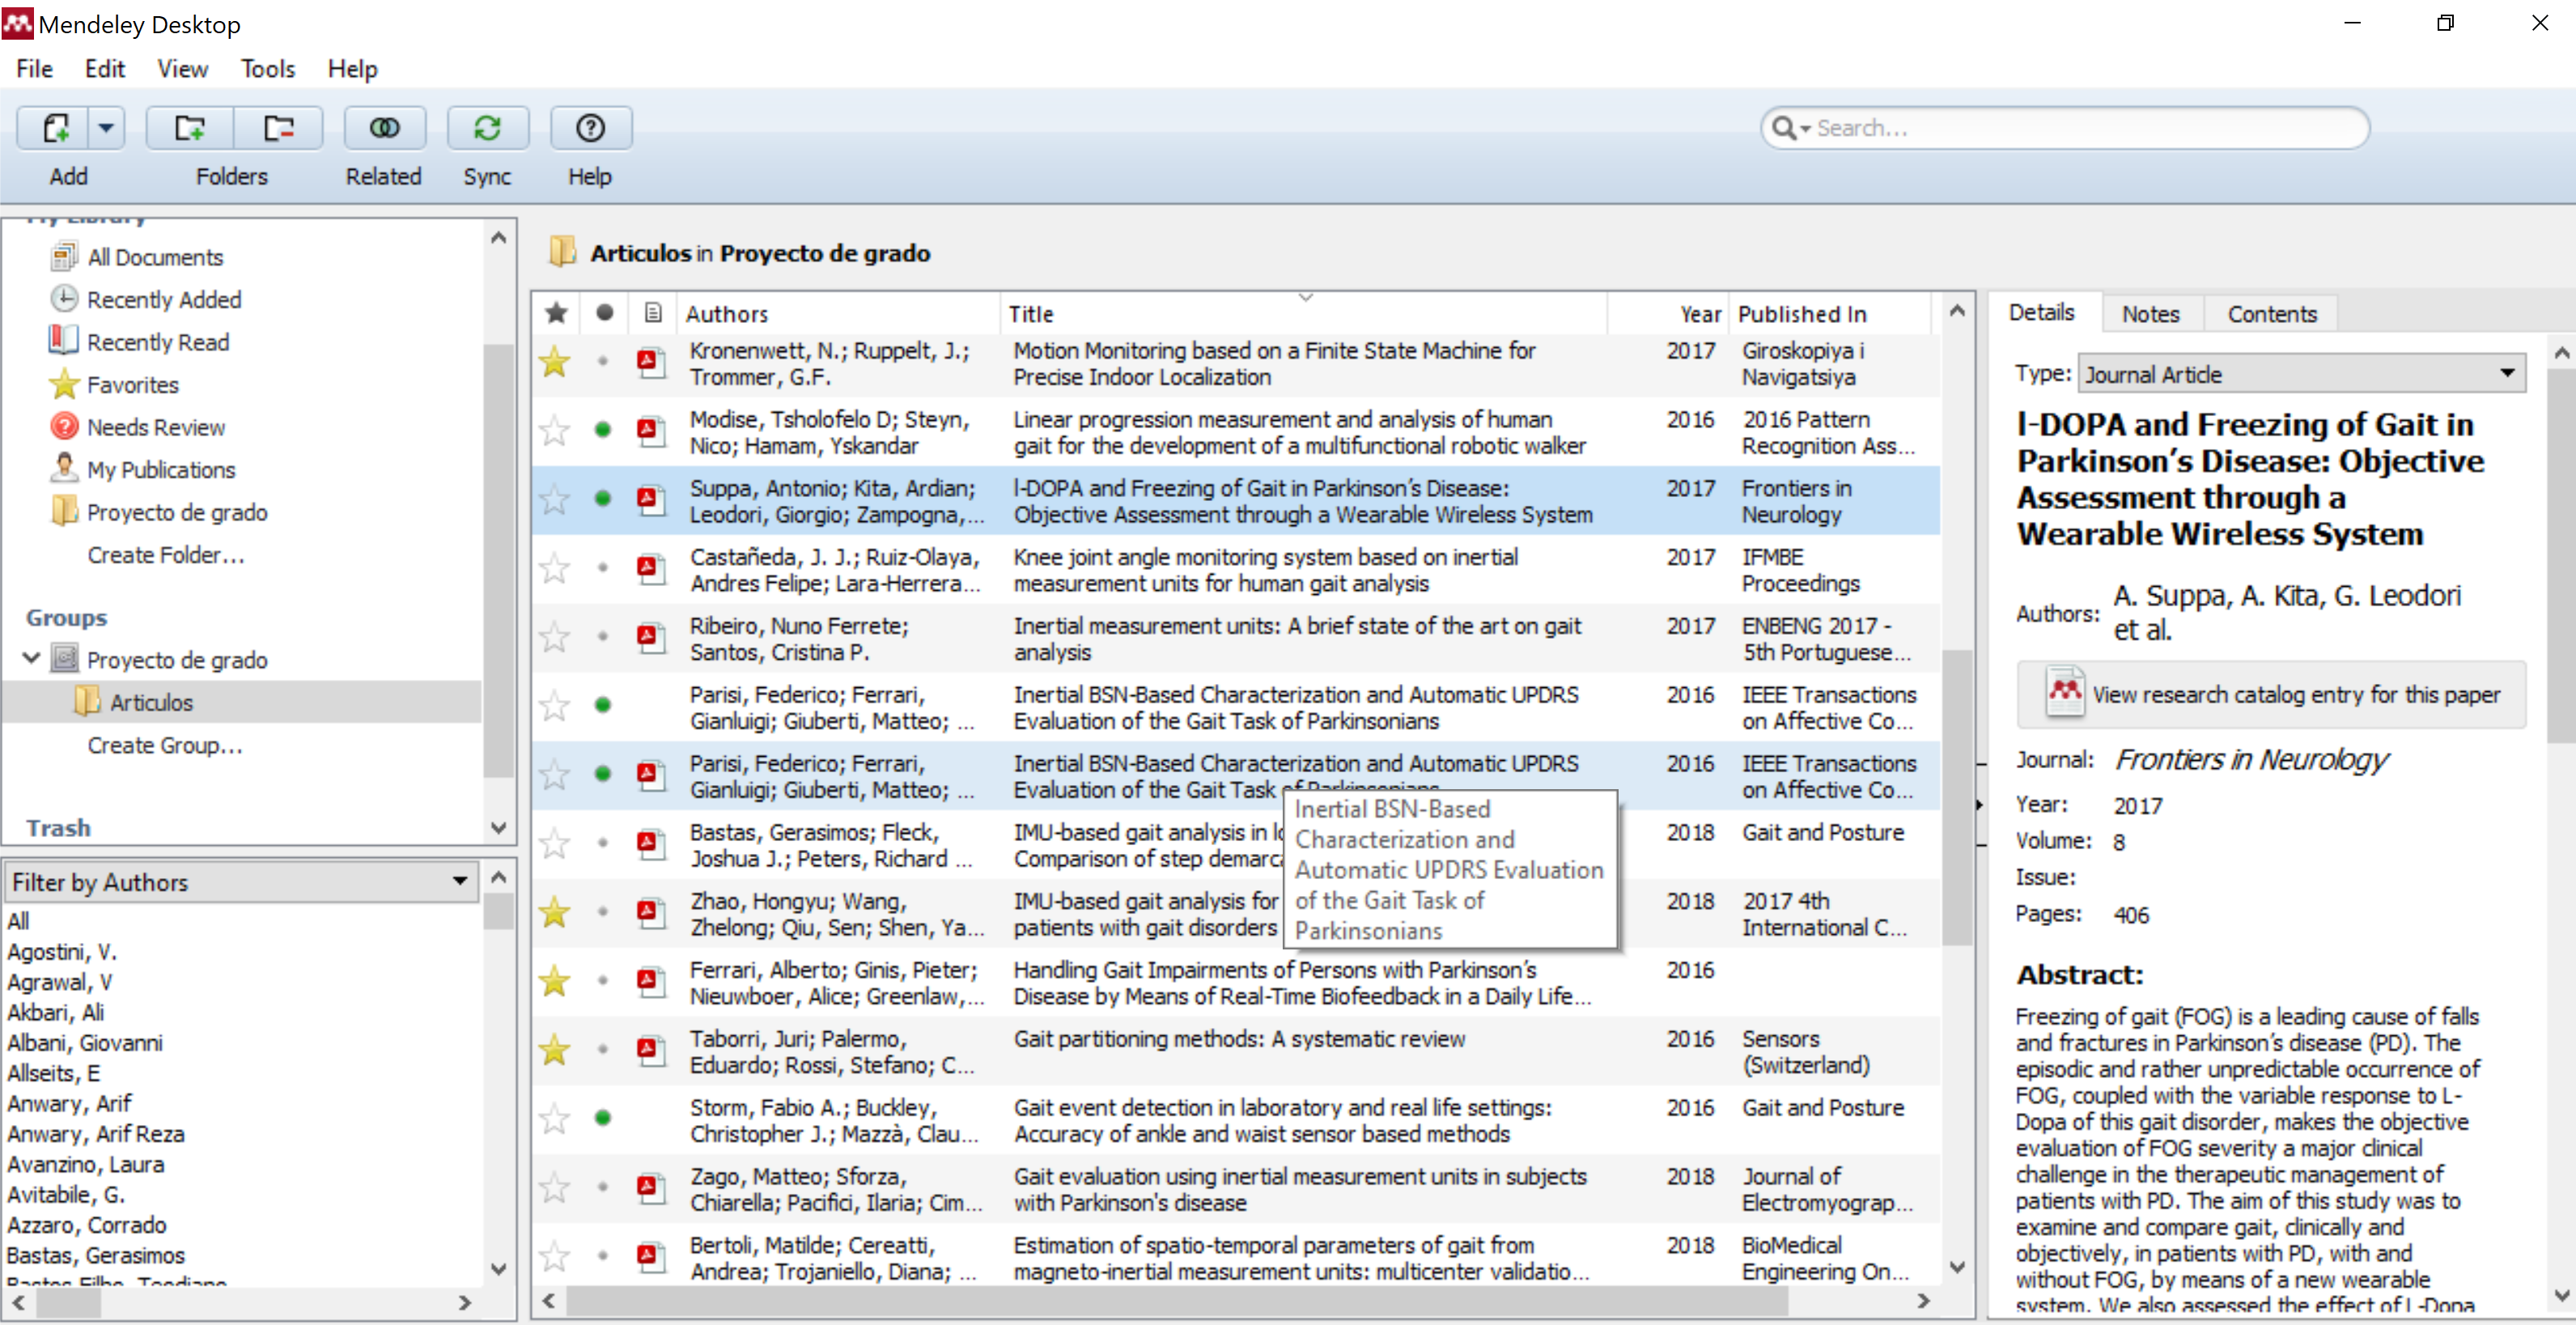
\includegraphics[width=\textwidth]{TESIS/imagenes/chap04/Mendeley.png}
\caption{ Gestor de referencias bibliográficas de PARKIBIP.}
\label{fig:admin_references}
\end{figure}

\section{Gestión de archivos}

En el transcurso del desarrollo del proyecto se generan y utilizan una gran variedad de archivos, tales como notas, actas de reuniones, documentos, planillas de cálculo, cuadros comparativos, imágenes, formularios, presentaciones, entre otros. Para gestionar estos archivos se utilizó la herramienta Google Drive (© Google LLC). Google Drive es un servicio de alojamiento de archivos en la nube que permite no solo almacenar documentos sino que también crear éste tipo de documentos (p. ej. documentos de texto, planillas de cálculo y presentaciones); para luego trabajar de manera colaborativa y sincronizada, es decir, con varias personas trabajando en un mismo documento y al mismo tiempo. Las unidades de almacenamiento pueden ser compartidas entre diferentes usuarios.

\section{Entorno de desarrollo}

% Android Studio 

Android Studio fue el \gls{IDE} (del inglés ``Integrated Development Environment'') que se utilizó para desarrollar la aplicación PARKIBIP. Es el IDE oficial por excelencia para el desarrollo de aplicaciones Android, basado en IntelliJ IDEA (© 2000-2020 JetBrains). Android Studio -desarrollado sobre el editor de código y herramientas de desarrollo de IntelliJ-,  ofrece todas las funcionalidades necesarias para construir aplicaciones Android, tales como:

\begin{itemize}
    \item Sistema de emuladores de dispositivos 
    \item ``Build system'' flexible basado en Gradle 
    \item Un entorno unificado para el desarrollo de aplicaciones para cualquier dispositivo
    \item Integración con herramientas de versionado de código 
    \item Plantillas de código utiles para desarrollar patrones comunes 
    \item Herramientas de Testing, etc.
\end{itemize}

\section{Versionado de código}\label{project:version-control}

Un sistema de control de versiones (a.k.a. VCS, ``Version Control System''), permite realizar un seguimiento de los cambios interactivos en la base de código \cite{Blischak2016}. De esta forma, se puede experimentar nuevas ideas con la opción de revertir esos cambios hacia una versión anterior. A través de un VCS se pueden adjuntar mensajes que describen cada una de las versiones, así como trabajar en distintas versiones de forma paralela, por lo que facilita la colaboración. Además, un colaborador puede aplicar ciertos cambios al código y otro puede rápidamente incorporar esos cambios. 
El VCS más popular actualmente es Git \cite{Blischak2016} y fue el elegido para el versionado de código en PARKIBIP. Git permite crear fácilmente ramas -versiones del código, esencialmente-. Esto significa que se puede configurar de manera segura una rama para cierto desarrollo, una rama para la codificación de proyectos experimentales, una rama para producción y una rama para cualquier otra cosa que sea necesaria. Al finalizar el desarrollo de cierto código, se puede fusionar una rama con otra, por ejemplo la de desarrollo a la de producción. 

En PARKIBIP se utilizó una rama de desarrollo llamada ``develop'' y una rama de producción llamada ``master'' como se muestra el esquema en la figura Fig. \ref{fig:branching-model}. Luego, para cada nueva funcionalidad se creó una rama con un nombre que describe la misma y un prefijo ``feature/'' -indicando que está creado con el propósito de desarrollar una funcionalidad-.

\begin{figure}[H]
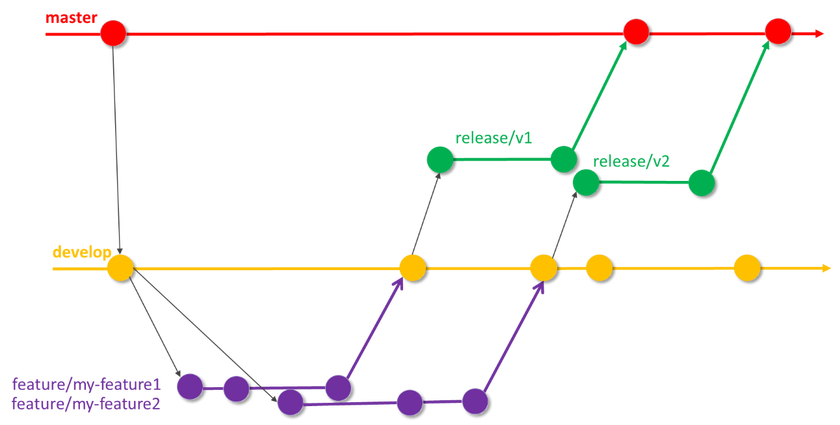
\includegraphics[width=\textwidth]{TESIS/imagenes/chap04/gitflow-branching-model.png}
\caption{ Modelo de ramas para flujo de trabajo en git  }
\label{fig:branching-model}
\end{figure}

Una vez terminado el trabajo de desarrollo en esa rama, se crea un \gls{merge_request} contra la rama de desarrollo, utilizando la herramienta Gitlab disponible gratuitamente para alumnos de la Facultad de Ingeniería. Dicha solicitud puede ser revisada por otro integrante del equipo, es decir, realizar comentarios, sugerencias o correcciones sobre los cambios que se están solicitando fusionar. Una vez que el otro integrante aprueba la fusión, la rama puede fusionarse para que la nueva funcionalidad esté disponible en la rama de desarrollo. 

De esta forma, es posible organizar las versiones del código de una forma estratégica, sencilla y efectiva. Cuando se quiere incorporar una corrección sobre una funcionalidad ya desarrollada, el proceso es el mismo pero el nombre de la nueva rama tiene el prefijo ``fix/''.

\section{Diagramas de diseño}

Para elaborar la documentación de diseño -arquitectura, modelado de procesos-, diagramas de componentes, diagramas de comunicación, diagramas de clase, etc. se utilizó la herramienta Microsoft Visio (© Microsoft 2020). Esta herramienta permite diseñar de manera sencilla e intuitiva diagramas de flujo, organigramas, diseños de ingeniería y todo tipo de diagramas en general. 

Fue utilizado principalmente para la elaboración de diagramas de flujo de actividades y datos, conocido como la notación BPMN 2.0 (Business Process Model and Notation), es decir, representaciones gráficas de flujos o procesos de negocio. De esta manera, el modelo permite visualizar de forma clara los eventos, actividades, actores, asociaciones y relaciones, tareas manuales o de sistemas, ``timers'' disparadores de acciones, y demás. Permite centralizar en un diagrama integrado todas las funcionalidades o historias de usuario del sistema.

\section{Documentación} 

Para la documentación del proyecto se utilizó la herramienta Overleaf (© 2020 Overleaf), un editor de LaTex en línea que permite escribir documentos científicos de forma colaborativa; es decir, que varios colaboradores puedan trabajar en el mismo documento al mismo tiempo. Es utilizada actualmente por cerca de cinco millones de investigadores, estudiantes y profesores en instituciones educativas (p.ej: Harvard, Oxford, entre otras), laboratorios y la industria en general. La herramienta se accesible a través de la web y permite, entre otras cosas:

\begin{itemize}
    \item Chat con personas que se encuentran trabajando en el mismo documento 
    \item Agregar comentarios a partes específicas del texto 
    \item Responder o resolver comentarios sobre el texto de otros colaboradores 
    \item Disponer de un historial de modificaciones 
\end{itemize} 

\section{Otras herramientas de desarrollo}

Como toda investigación y experimentación, siempre es necesario la realización de Pruebas de Concepto (POC, del ingles Proof of concept) que permitan experimentar funcionalidades de una manera rápida y temprana, como también reducir incertidumbres.

Por lo tanto, fueron utilizadas diversas herramientas, como por ejemplo VisualStudio y el lenguaje .NET, Python, Bosch Development Desktop 2.0, etcétera. Principalmente para las actividades:

\begin{itemize}
    \item Envío y recepción de eventos hacia/desde los dispositivos IMU.
    \item Recuperación de datos medidos por los sensores.
    \item Computo de algoritmos numéricos.
    \item Implementación de otros métodos o técnicas (i.e. algoritmo de fusionado y filtrado de datos, computo de orientación).
\end{itemize}